\section{Related Works}
\subsection{Evolution of YOLO Detectors}
Since the advent of deep convolutional neural networks~\cite{survey_20y}, real‑time object detection has rapidly evolved from multi‑stage pipelines exemplified by the R‑CNN series~\cite{rcnn,fast_rcnn,faster_rcnn, maskrcnn} to highly optimized single‑stage frameworks epitomized by the YOLO models~\cite{yolo_survey}. The original YOLO (You Only Look Once) model~\cite{yolov1} first recast detection as a single‑shot regression problem, eliminating proposal‑generation overhead and achieving an excellent speed-accuracy trade‑off. Subsequent YOLO iterations have continually refined architecture and training strategies~\cite{yolo_based_survey,yolo_survey}. YOLOv2~\cite{yolov2} boosted precision by introducing anchor‑based predictions and a DarkNet‑19 backbone. YOLOv3~\cite{yolov3} strengthened small‑object detection with a DarkNet‑53 backbone and three‑scale predictions. YOLOv4 through YOLOv8~\cite{yolov4,yolov5,yolov6,yolov7,yolov8} progressively integrated modules such as CSP, SPP, PANet, multi‑mode support, and anchor‑free heads to further balance throughput and accuracy. YOLOv9~\cite{yolov9} and YOLOv10~\cite{yolov10} then focused on lightweight backbones and streamlined end‑to‑end deployment. Later, YOLO11~\cite{yolo11} preserved the ``backbone-neck-head'' modular design but replaced the original C2f block with the more efficient C3k2 unit and added a Convolutional Block with Partial Spatial Attention (C2PSA) to enhance detection of small and occluded targets. The latest YOLOv12~\cite{yolov12} marks the full integration of attention mechanisms, introducing the Residual Efficient Layer Aggregation Network (R‑ELAN) alongside lightweight Area Attention (A2) and Flash Attention to optimize memory access, thereby achieving efficient global and local semantic modeling while maintaining real‑time performance and improving robustness and precision.

% PP‑YOLO~\cite{ppyolo} replaces the backbone with ResNet50‑vd‑dcn and incorporates IoU‑aware confidence scoring and DropBlock to elevate both accuracy and efficiency. 
Meanwhile, some YOLO‑based variants have emerged~\cite{yolo_survey}. YOLOR~\cite{yolor} fused explicit and implicit features for richer representations and stronger generalization. YOLOX~\cite{yolox} employed an anchor‑free head with dynamic label assignment to simplify the pipeline and improve small‑object detection. YOLO‑NAS~\cite{yolonas} leveraged AutoNAC for neural architecture search, using Quant‑Aware RepVGG and mixed‑precision quantization to optimize throughput and small‑object performance. Gold‑YOLO~\cite{goldyolo} introduced a GD mechanism to enhance multi‑scale feature fusion capabilities. YOLO-MS~\cite{yoloms} introduced an MS-Block with integrated Global Query Learning for dynamic multi-branch feature fusion and a progressive Heterogeneous Kernel Size Selection strategy to enrich multi-scale representations with minimal overhead.

However, as mentioned above, the architecture of the current YOLO series models limits them solely to modeling local pairwise correlations, preventing them from modeling global multi-to-multi high-order correlations. This restricts the detection performance of existing methods in complex scenarios.

\begin{figure*}[!tp]
    \centering
    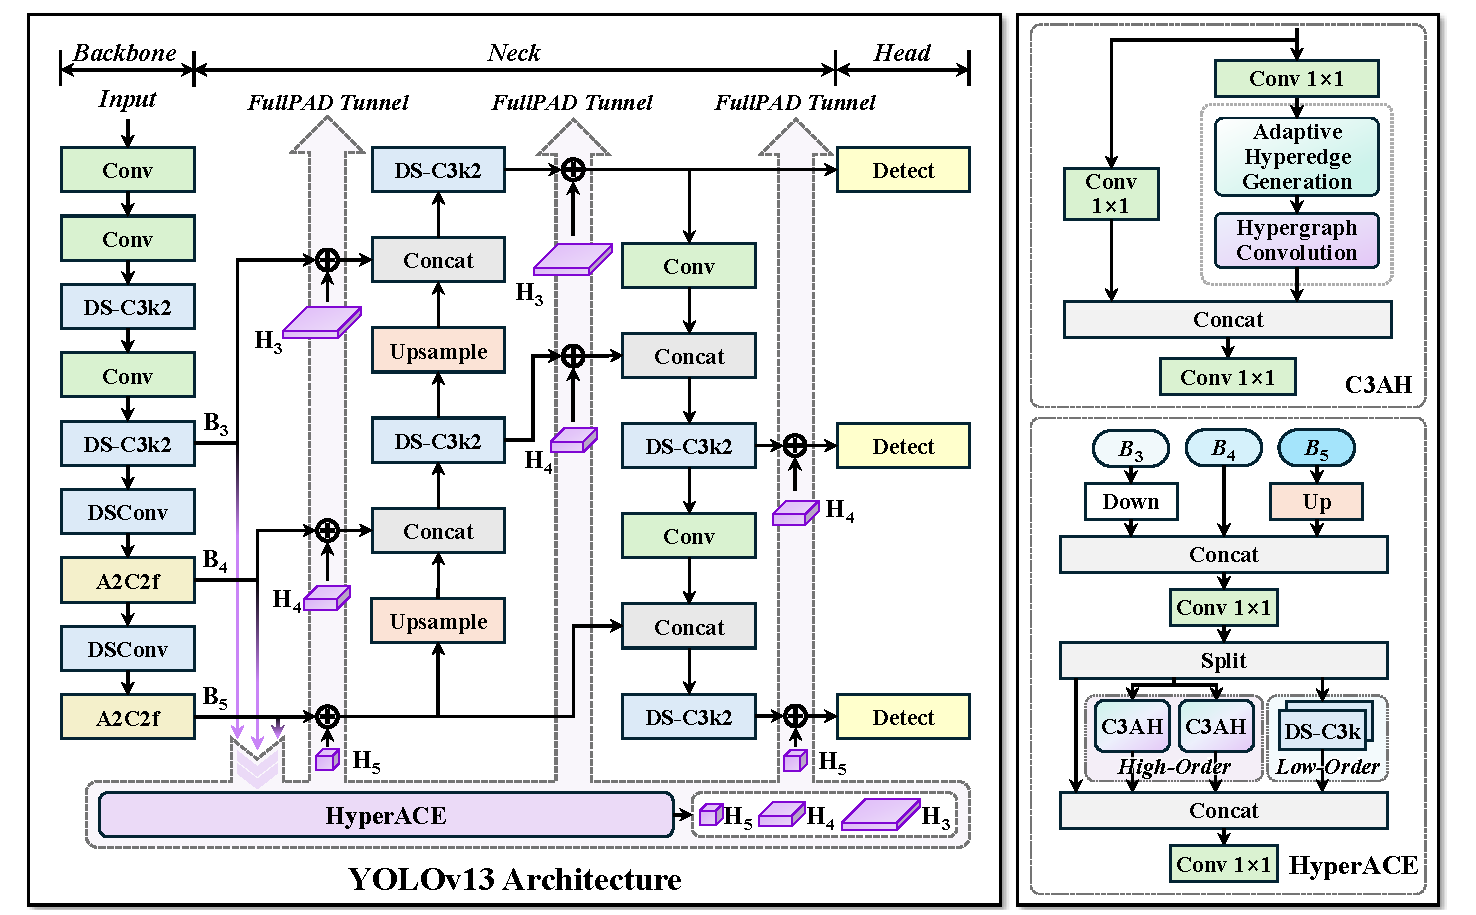
\includegraphics[width=0.9\linewidth]{figures/framework.pdf}
    \vspace{-0.2cm}
    \caption{The network architecture of our proposed YOLOv13 model. Taking multi-scale features extracted from the backbone as input, HyperACE adaptively explores high-order correlations and achieves feature enhancement and fusion. Then, the correlation-enhanced features are distributed to the entire network by FullPAD tunnels to achieve accurate object detection in complex scenes. The detailed structure of HyperACE is shown on the right.
    % The right part is the structure of the Hypergraph-based Adaptive Correlation Enhancement (HyperACE) mechanism. The upper right shows the C3AH used in HyperACE.
    }
    \vspace{-0.2cm}
    \label{fig:framework}
\end{figure*}


\subsection{High-Order Correlation Modeling}
Complex multi-to-multi high-order correlations are ubiquitous in nature, \eg, neural connections and protein interactions, as well as in the field of information science, \eg, social networks~\cite{hg_book, hg_learning}. In visual data, different objects engage in spatial, temporal, and semantic interactions forming complex correlations. These correlations may be pairwise (low‑order) or more complex group‑based correlations (high‑order).
% For example, at the macroscopic level, multiple objects interacting within the same scene form a high‑order association; at the microscopic level, pixels jointly contributing to a visual feature can also constitute a high‑order association. 
Hypergraphs, the extension of vanilla graphs, can represent not only pairwise correlations but also multi‑to-multi high‑order correlations~\cite{hg_survey,hg_survey2}. In recent years, hypergraph neural networks (HGNNs) have emerged as a primary tool for modeling such high‑order correlations~\cite{hg_derain,hg_medical,hg_network,hyperyolo}. Feng~\etal~\cite{hgnn} proposed spectral‑domain HGNNs, demonstrating the advantage in the visual retrieval task. Gao~\etal~\cite{hgnnp} further proposed HGNN$^+$ with spatial hypergraph convolution operators, enhancing HGNN applicability.
% and Lei et al. \cite{softhgnn} formulated the concept of soft hypergraphs, using a differentiable participation matrix to capture soft node associations that better reflect the inherent fuzziness of real-world visual data. However, modeling high‑order visual correlations remains largely unexplored in existing object detection frameworks. 
Recently, Feng~\etal\cite{hyperyolo} pioneered the integration of HGNN into detection models, demonstrating the necessity of high-order correlation modeling for detection. However, this method simply uses a handcrafted fixed parameter as threshold, and pixels with feature distances smaller than the threshold are determined to be correlative, leading to inadequate correlation modeling accuracy and robustness.

To address the above-mentioned challenges, we propose a hypergraph-based adaptive correlation enhancement mechanism, which efficiently models cross-location and cross-scale semantic interactions by adaptively exploiting latent correlations. This mechanism overcomes the lack of robustness in existing hypergraph computing paradigms caused by handcrafted hyperparameters, as well as the absence of global high-order correlation modeling in existing YOLO series models.
% fill this gap by introducing a soft hypergraph‑based visual association capturing module that efficiently models cross‑position and cross‑scale semantic interactions with linear complexity, thereby addressing the lack of high‑order association modeling in the YOLO family. In the next section, we delve into the specific design of YOLOv13.